\documentclass[../summary.tex]{subfiles}

\begin{document}
\section{Demography}
\subsection{Introduction}
\subsubsection{Population growth}

The global population has experienced a remarkable and rapid increase in recent history, but this growth has raised concerns about the Earth's capacity to sustain such numbers. Looking at the historical trajectory, we see that for most of human existence (approximately 300,000 years), the population remained relatively low, with just tens of millions of people on the planet. However, in the last 200 years, there has been an unprecedented surge, bringing the global population to around 8 billion.

\begin{figure}[H]
	\centering
	\begin{subfigure}{.5\textwidth}
		\centering
		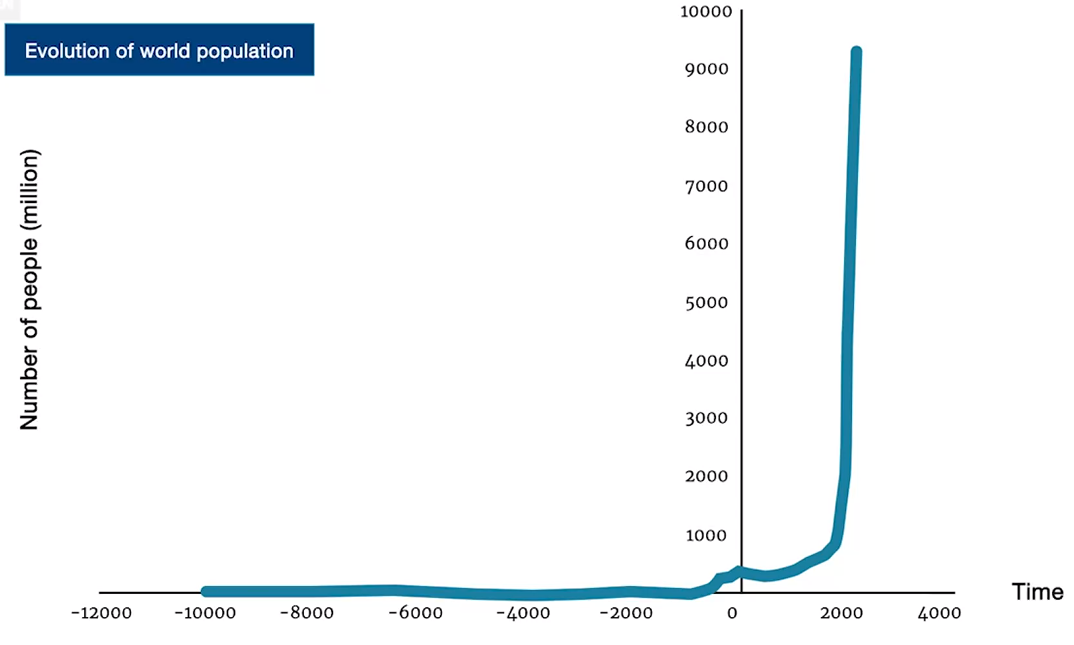
\includegraphics[width=1\linewidth]{../images/evolution_of_population}
		\caption{}
		\label{fig:evoltionofpopulation2}
	\end{subfigure}%
	\begin{subfigure}{.5\textwidth}
		\centering
		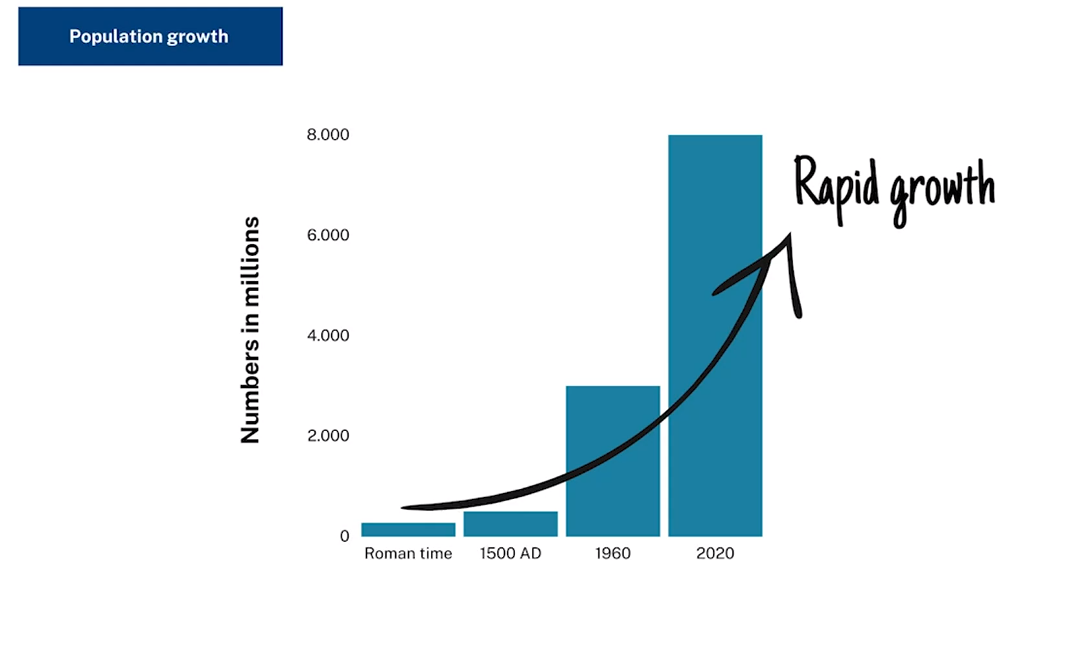
\includegraphics[width=0.9\linewidth]{../images/evolution_of_population_2}
		\caption{}
		\label{fig:evoltionofpopulation3}
	\end{subfigure}
	\caption{Evolution of the world population}
	\label{fig:evoltionofpopulation}
\end{figure}

\ \\
This rapid growth is a cause for concern for many, as some fear that it may lead to unsustainable pressure on the planet's resources and potential societal collapse. Reverend Thomas Malthus in the late 18th century and Paul Erlich in the 1960s both predicted such scenarios based on population growth.\\
\\
However, simply extrapolating from the past isn't sufficient to predict the future accurately. To gain a deeper understanding and insight, we must examine the mechanisms responsible for this recent population surge. We need to determine whether these mechanisms will continue to drive rapid population growth or if there are factors that may slow it down. By understanding these mechanisms, we can make informed projections and consider potential interventions to manage and control population growth.\\
\\
In essence, addressing the issue of population growth requires a scientific approach. We must delve into the historical and current factors driving population growth and use this knowledge to make more informed predictions about the future. This approach allows us to explore questions about the world's population in the coming decades and consider strategies to manage and reduce growth if deemed necessary.
\newpage

\subsection{History of mortality}
\subsubsection{Exponential growth}

Exponential growth is a fundamental concept often used to explain pessimistic views regarding population growth. It can be likened to the compound interest calculation used by banks, where a fraction of the existing capital is added each year. This results in a growing fraction being added as the total increases, leading to a rapidly accelerating growth curve.\\
 \\
Exponential growth is not confined to banking; it is observed in various aspects of life, including the spread of diseases like COVID-19, where the number of cases can grow exponentially. The key properties of exponential growth are its potential to reach any number, as there's no fixed limit, and acceleration over time.\\
\\
Critics of population growth point to this concept to express concerns about the Earth's capacity to sustain an ever-growing population. For instance, they argue that if each family has a certain number of children, and this pattern continues from one generation to the next, it would result in exponential population growth. However, this simplistic view doesn't account for the complexities of real-world demographics and population dynamics.\\
\\
To examine the issue, we should analyse population trends on a global scale over longer time periods, which can reveal whether growth is truly exponential or even more rapid, referred to as "super-exponential growth" .  On figure \ref{fig:evolutionoftheglobalpopulation}, the population is on a logarithmic axis. The population evolution does not plot as a straight line, but as a curve that is bending upwards. This means that the global population is growing even faster than exponential growth predicts. 
 
 \begin{figure}[H]
 	\centering
 	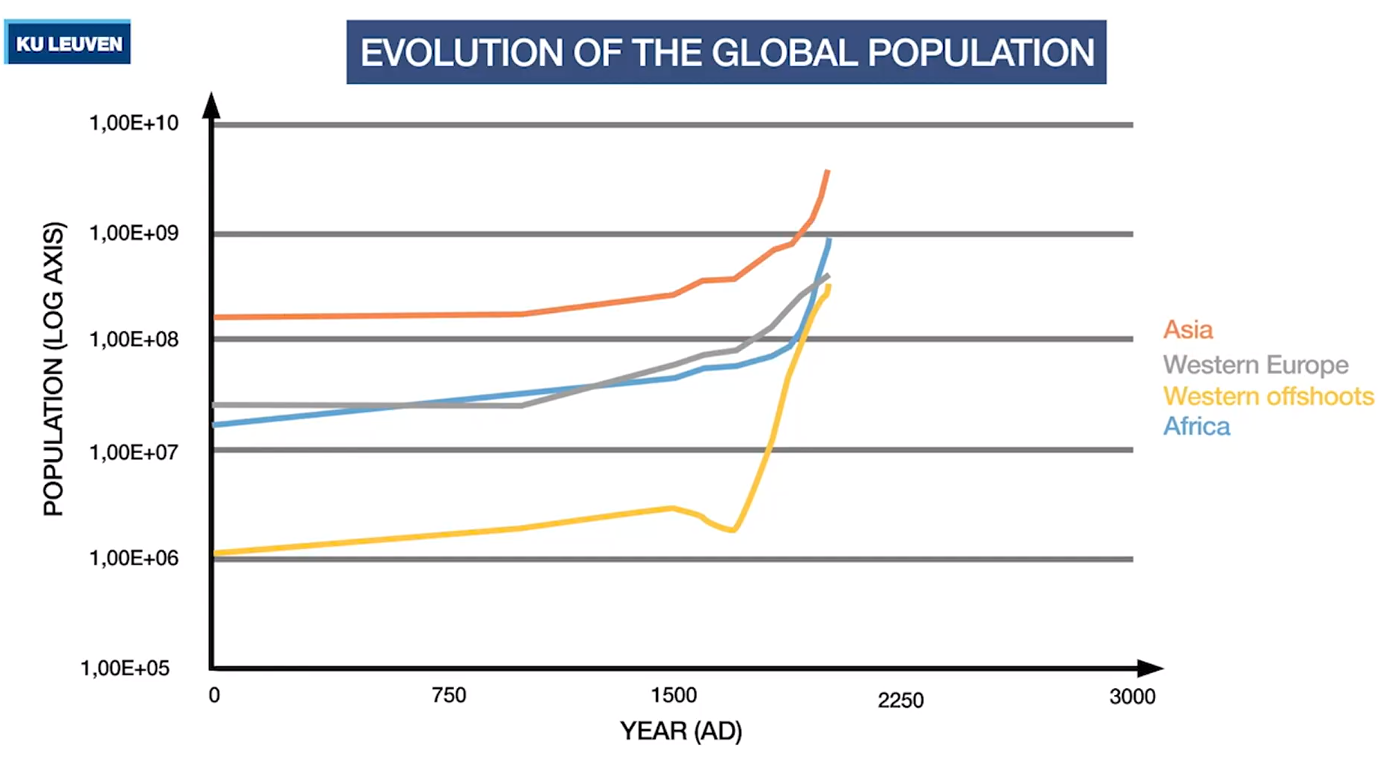
\includegraphics[width=0.8\linewidth]{../images/evolution_of_the_global_population}
 	\caption{Evolution of the global population}
 	\label{fig:evolutionoftheglobalpopulation}
 \end{figure}
 
 \ \\
 The latter is often seen as a potential crisis, as it can strain the capacity of systems to support the growing population. This leads to questions about whether the Earth can sustain such rapid growth, and if we can simply extrapolate past trends into the future.\\
 \\
 If we were to assume a 1\% annual growth rate, the Earth's population could exceed 20 billion people by the year 2122. This raises concerns about the planet's ability to support such a population. However, it's essential to consider whether this exponential growth will indeed persist, or if other factors and mechanisms will come into play to slow down population growth. This question remains a topic of ongoing research and debate.

\subsubsection{Industrial revolution}

The Industrial Revolution, which began in the 18th century, brought about significant changes in society and had a profound impact on health and mortality rates. Contrary to common perception, the introduction of industrialization led to a remarkable decline in mortality rates.\\
\\
Mortality rates in England, as well as in other countries experiencing the Industrial Revolution, started to decline from the very beginning of this transformation. Over a span of approximately 150 years, \textbf{mortality rates} in Great Britain were \textbf{halved}. This trend was not limited to one region; similar patterns emerged in countries undergoing industrialization.\\
\\
The key driver behind this decline in mortality was the increase in the availability of energy. The Industrial Revolution enabled society to extract more energy from the environment, which, in turn, transformed the mode of production and led to significant societal development.\\
\\
The availability of energy played a pivotal role in driving this transformation. To illustrate the magnitude of change, a single person working in a mine for a year could produce as much energy as is contained in a small jerrycan of diesel. That jerrycan represents just a fraction of the energy required to fuel a car. The vast increase in available energy fundamentally altered society.

\begin{figure}[H]
	\centering
	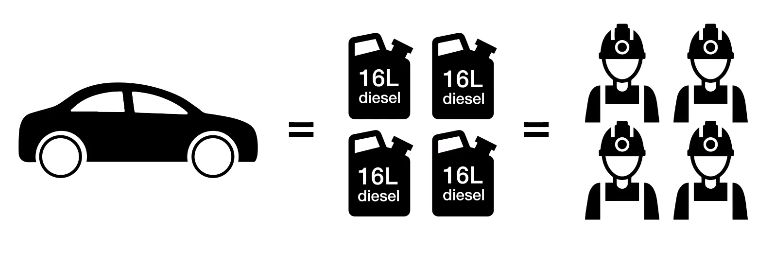
\includegraphics[width=0.7\linewidth]{../images/mine_worker}
	\caption{Energy comparison}
	\label{fig:mineworker}
\end{figure}
\ \\
The mode of production shifted from a predominantly rural setting where people worked on farms to an industrial society characterized by factories and machinery powered by fossil fuels. Workers in factories were initially inexperienced and required training. Factory owners who invested in training their workforce realized higher productivity and safety. Over time, those who provided training outperformed competitors who did not.\\
\\
Education and training provided not only the skills necessary for employment but also additional skills that improved individuals' abilities to reflect, discuss, understand their health, follow medical treatments, express their needs, and plan families. This marked a significant shift in society's capabilities.\\
\\
As industrialization progressed, society reorganized itself. Cities grew in importance, religion played a reduced role, and unions formed as workers could now collectively negotiate with factory owners. The demand for knowledge and technological advancement to improve efficiency in factories led to the development of science and technology. These advancements were not confined to industry but also extended to areas like healthcare, food production, and administrative efficiency (figure \ref{fig:reorganisationsociety}).

\begin{figure}[H]
	\centering
	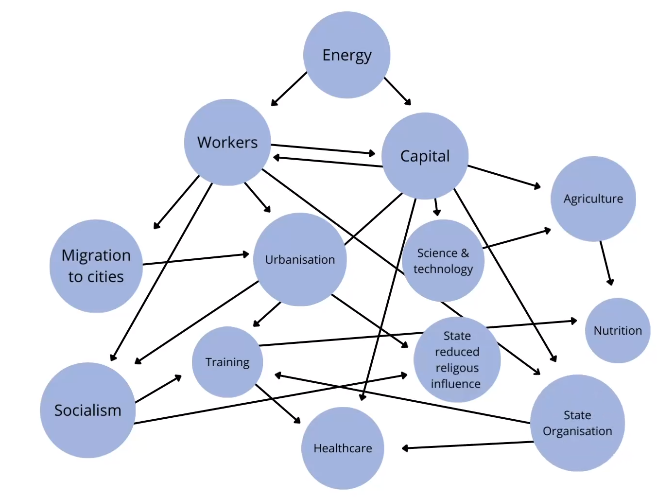
\includegraphics[width=0.7\linewidth]{../images/reorganisation_society}
	\caption{Reorganisation of the society since the industrialization}
	\label{fig:reorganisationsociety}
\end{figure}
\ \\
This combination of increased knowledge, societal organization, and technological advancements contributed to a dramatic reduction in mortality rates. The Industrial Revolution was not a detriment to health but, in fact, a driver of increased life expectancy and overall well-being.

\subsubsection{Relation longevity - mortality}

In population dynamics we often speak of mortality. This number indicates how many people die in a given year, but this number also gives you information on the live expectancy of the population. In a population with a high mortality, you will probably not live very long.\\
\\
In equilibrium, the average lifespan is simply the inverse of the mortality. So, when the mortality is 30\textperthousand, 30 out of 1000 people will die in a given year.  You can calculate the lifespan as follows:\\
\[lifespan = mortality^{-1} = \left(\frac{30}{1000}\right)^{-1} = \frac{1000}{30} = 33\ years\] 
\newpage
\subsubsection{Mortality decline}

During the Industrial Revolution, various factors contributed to a dramatic decline in mortality rates, resulting in a significant increase in life expectancy. Several key elements played crucial roles in this transformation:
\begin{itemize}
	\item \textbf{Advancements in Medicine:} The development of the first vaccines in the 18th century, particularly the smallpox vaccine, significantly reduced mortality. Lady Montagu introduced the practice of inoculation from Turkey to Europe, and later, Jenner created a safe smallpox vaccine using cowpox scabs.
	\item \textbf{Sanitation Improvements:} Observations and empirical evidence, such as John Snow's investigation during a cholera outbreak, led to the understanding of waterborne diseases. Closing contaminated water sources helped prevent the spread of diseases and reduced mortality.
	\item \textbf{Government Initiatives:} Governments took action to improve sanitation. In London, the construction of precipitation works in the 1860s addressed the pollution of the River Thames, contributing to cleaner water and a decrease in disease risks.
	\item \textbf{Food Safety Measures:} Sterilization of foods, a practice developed around 1810, became a critical factor in reducing the risk of food poisoning. Cooking and sterilizing food allowed for longer preservation and safer consumption.
	\item \textbf{Increased Food Production:} Scientific advancements, particularly by German chemist von Liebig, provided insights into plant growth and the role of nutrients. This knowledge allowed for increased food production, ensuring a more abundant and varied diet.
	\item \textbf{Healthcare Systems:} The establishment of healthcare systems, starting with Otto von Bismarck's sick law in Germany, provided support to individuals during periods of illness. Sick funds, funded by employer and employee contributions, helped protect the population's health.
	\item \textbf{Educational Improvements:} The rise of education, with an increasing percentage of the population attending school, played a vital role. Better-educated individuals were more capable of understanding and adhering to health-related practices, contributing to overall well-being.
\end{itemize}
\ \\
The combination of these factors, rather than any single measure, led to a substantial reduction in mortality rates and a doubling of life expectancy during the Industrial Revolution. The societal changes, improvements in knowledge, and the organization of society were fundamental drivers of this remarkable increase in life expectancy. Importantly, this increase was not solely dependent on wealth, as demonstrated by the fact that societal changes had a more significant impact on life expectancy than the absolute wealth of a country.

\subsubsection{Spread of mortality decline}

The demographic transition starts with a the decline of mortality: there is no country in the world where fertility declined before mortality declined.\\
\\
The very first country that saw a mortality decline was England, where the Industrial Revolution started: mortality started to decline here at the moment the Industrial Revolution started, i.e. the 2nd half of the 18th century.  The decline of mortality then followed for some time the spread of the Industrial Revolution: the first countries that followed in the first half of the 19th century were European countries like Belgium and Sweden as well as the United States and Canada, with Germany following somewhat later.  Further East (in Russia) and South mortality started to decline at the end of the 19th or the beginning of the 20th century.  Most of the rest of Asia and Latin America saw the beginning of the mortality decline after WW1 and it was only after WW2 that the decline started in earnest in Sub-Saharan Africa. 

\begin{figure}[H]
	\centering
	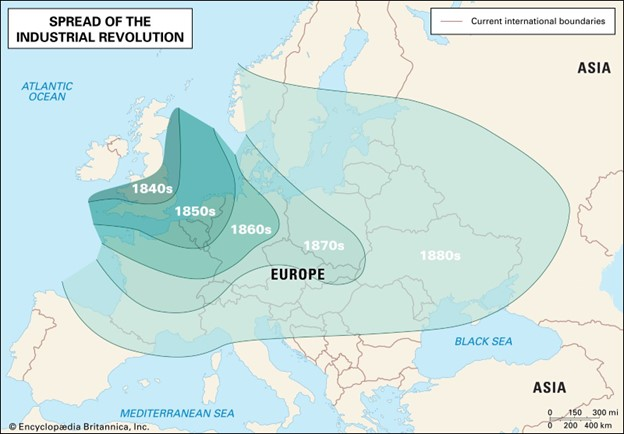
\includegraphics[width=0.7\linewidth]{../images/spread_of_industrial_revolution}
	\caption{Spread of the industrial revolution}
	\label{fig:spreadofindustrialrevolution}
\end{figure}

\subsection{History of fertility}
\subsubsection{Timing of fertility decline}

In general the decline of fertility starts decades after the decline of mortality. Society has to adjust to a higher life expectation before this higher life expectation translates into a lower number of children being born. \\
\\
Fertility started to decline in England by the end of the 19th century, ca. 100 years after the start of the mortality decline. Other countries in Western Europe as well as the United States and Canada followed quickly. Further South (Mediterranean Europe) and East (Russia) saw a decline in mortality from the beginning of the 20th century with most of Asia and Latin America following suit after WW2. In Sub-Saharan Africa however, fertility only started to decline in earnest after 1990. \\
\\
\textbf{The French exception}\\
In nearly all countries fertility only started to decline decades after mortality decreased but there is one notable exception to this rule. In France both mortality and fertility started to decline at the end of the 18th century, making France the first country where the number of children being born started to fall. There is still a scientific debate as to why this happened but it is very tempting to consider the French Revolution of 1789 to be at least an important contributing factor. The French Revolution upended the feudal society that France was up to that point of time and stressed not only freedom, equality and solidarity but also autonomy, thereby creating an environment wherein young families could make their own decisions. Families responded by rapidly reducing the number of children they had resulting in a far lower population growth in France during the demographic transition in comparison to other European countries.
\newpage

\subsubsection{Fertility and child mortality}

\textbf{Why was fertility so high before the industrial revolution?}\\
Before the industrial revolution, societies were primarily agrarian and rural. People's livelihoods depended heavily on agriculture, and they lacked the social and economic structures that characterize modern industrial societies. Several factors contributed to high fertility rates during this period:
\begin{itemize}
	\item \textbf{High Child Mortality:} Child mortality rates were significantly high, often around 50\% or more. With the lack of advanced healthcare and sanitation, many children did not survive to adulthood.
	\item \textbf{Economic Dependence on Children:} In the absence of pensions, healthcare, and social security systems, elderly individuals relied on their children for support in old age. Having more children increased the likelihood that at least some would survive to provide care and support.
	\item \textbf{Agrarian Economy:} In rural, agrarian societies, large families were often seen as economic assets. Children could contribute to farm work and family income from a young age, helping to sustain the household.
	\item \textbf{Risk Mitigation:} Parents had more children to mitigate the risk of losing some to mortality. The unpredictability of survival meant that families had to have more children to ensure the presence of adult offspring to care for them.
\end{itemize}
\ \\
\textbf{Why did fertility decline after the industrial revolution?}\\
The industrial revolution brought about significant societal changes, including advancements in healthcare, technology, and the nature of work. These changes influenced a decline in fertility rates:
\begin{itemize}
	\item \textbf{Reduced Child Mortality:} With improvements in healthcare, sanitation, and overall living conditions, child mortality rates drastically decreased. Parents no longer needed to have a large number of children to ensure that some would survive to adulthood.
	\item \textbf{Shift in Economic Structure:} The shift from agrarian to industrial economies meant that the economic role of children changed. Instead of being contributors to family income through labour on farms, children became recipients of education and needed more resources for their development.
	\item \textbf{Social Welfare Systems:} The emergence of social welfare systems, including healthcare and pensions, meant that elderly individuals were no longer solely dependent on their children for support. This reduced the need for large families to ensure care in old age.
	\item \textbf{Educational Investments:} Industrial societies placed a higher value on education. Parents began investing more time and resources in the education of their children, aiming for quality rather than quantity.
	\item \textbf{Changing Role of Women:} As industrialization progressed, women increasingly participated in the workforce. This shift, combined with the desire for personal and professional development, led to delayed marriages and childbirth, contributing to lower fertility rates.
\end{itemize}
\newpage

\subsection{Future prospects}
\subsubsection{Factors influencing fertility decline}

The key to reducing fertility rates lies in addressing various factors. Child mortality, a crucial factor, must be reduced, even though it may seem counterintuitive, as lower child mortality is linked to lower population growth. Progress has been made globally, with child mortality now well below 10\% in most countries, and efforts to further decrease it are underway, particularly in sub-Saharan Africa. It is possible to reduce child mortality everywhere around the world below 2\% and we are on track of doing so.\\
\\
Besides child mortality, other factors contribute to fertility rates. Wealthier societies tend to have fewer children, and there's a correlation with the age at which women marry. However, the most significant correlation is with the education of women. Educated women tend to use contraception more effectively, delay childbearing while studying, and invest heavily in their children's education because they want that  their children have at least the same possibilities than they have had. This leads to a more rapid reduction in the number of children.\\
\\
While contraception plays a role, its impact varies. Historical examples, like Belgium before World War II, show fertility decline without modern contraception (figure \ref{fig:childrenperwoman}). 

\begin{figure}[H]
	\centering
	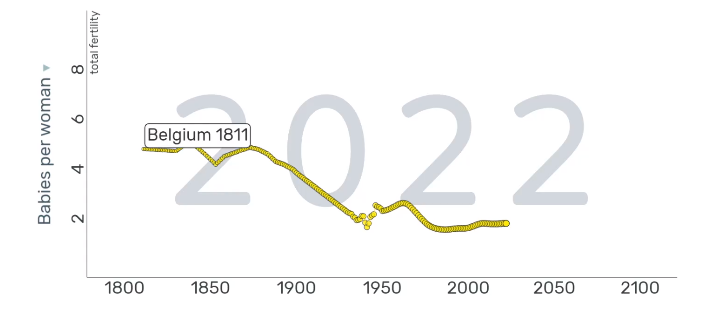
\includegraphics[width=0.7\linewidth]{../images/children_per_woman}
	\caption{Amount of children per woman in Belgium}
	\label{fig:childrenperwoman}
\end{figure}
\ \\
In developing countries, many women express a desire for fewer children than they actually have, indicating "unwanted fertility." Access to contraception and proper information can rapidly decrease unwanted fertility (figure \ref{fig:unwantedfertility}).

\begin{figure}[H]
	\centering
	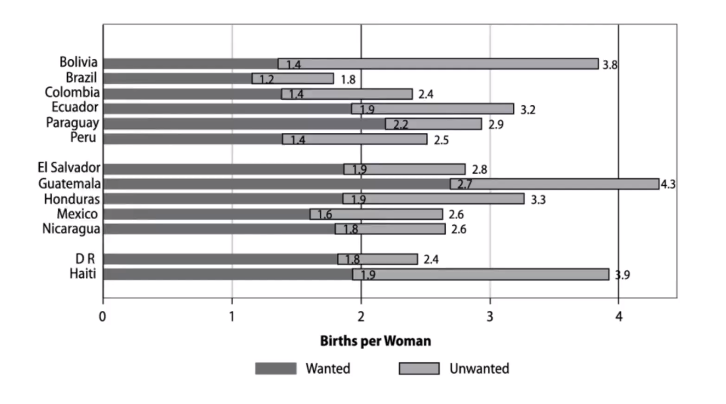
\includegraphics[width=0.7\linewidth]{../images/unwanted_fertility}
	\caption{Unwanted fertility in developing countries}
	\label{fig:unwantedfertility}
\end{figure}

\ \\
The process of fertility decline is inherently slow due to cultural and social norms. Unlike mortality decline, which is universally desired, fertility is influenced by societal expectations. Changing cultural norms takes time, and efforts to stimulate fertility decline should acknowledge this. It's crucial to invest in reducing child mortality, educating women, and accepting the gradual nature of cultural change in order to achieve sustained fertility decline, especially in the global south.

\subsubsection{Rate of fertility decline}

Fertility decline is a slow, socio-cultural process while decline in child mortality depends more on the available knowledge and technical solutions (such as healthy food, medicine, …). Although these general processes are true for all countries, there are regional variations in the speed of mortality and fertility decline (figure \ref{fig:years-it-took-fertility-to-fall-from-6-to-below-3}).

\begin{figure}[H]
	\centering
	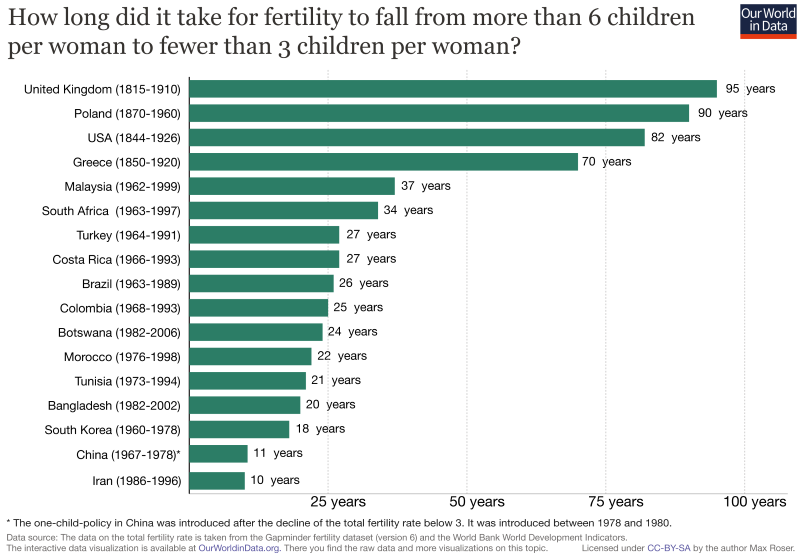
\includegraphics[width=0.7\linewidth]{../images/Years-it-took-Fertility-to-fall-from-6-to-below-3}
	\caption{Years it took for fertility to fall from more than 6 to less than 3 children per woman}
	\label{fig:years-it-took-fertility-to-fall-from-6-to-below-3}
\end{figure}
\ \\
In developed countries, birth and death rates were already somewhat lower before the start of the Industrial Revolution. The decline of mortality was slow, because technologies and knowledge were still begin developed. The following decline in mortality was slow as well. As you can see in figure , this leads to a population increase which is relatively small.

\begin{figure}[H]
	\centering
	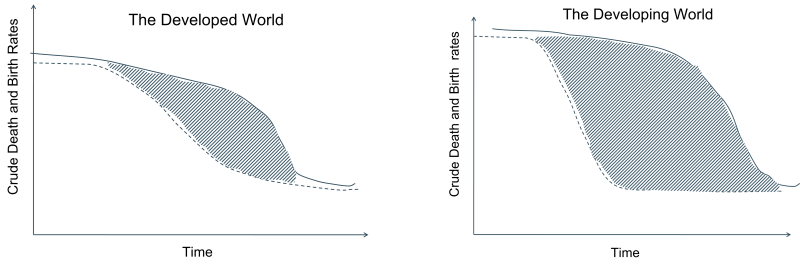
\includegraphics[width=0.8\linewidth]{../images/Fertility_and_mortality_decline_in_developed_vs_developing_countries}
	\caption{Fertility and mortality decline in the develop(ed)(ing) world}
	\label{fig:fertilityandmortalitydeclineindevelopedvsdevelopingcountries}
\end{figure}
\ \\
In the developing countries, birth and death rates were very high when the industrial revolution and societal transformation reached them. The knowledge to reduce mortality was already much more developed by then, leading to a much quicker decline in mortality. Fertility however, being a more socio-cultural process, is still a slow process. In the graph you can see how the combination of a fast mortality decline and slow fertility decline leads to a much larger population increase.

\subsubsection{Ageing}

The demographic transition follows a pattern where mortality decreases first, followed by a decline in fertility. During the initial phase of low mortality and high fertility, societies experience significant economic growth, as a large population of young adults contributes to economic development without the burden of caring for many older individuals. Examples include post-World War II Western societies and China between 2005 and 2020.\\
\\
This phase of economic growth is not guaranteed and requires effective economic policies, with education playing a crucial role. Investment in education is vital to develop the skills and knowledge needed for sustained economic development.\\
\\
However, as the demographic transition progresses, societies eventually age, with fewer young children and a larger population of older individuals requiring care and medical assistance. This shift poses challenges to economic growth, resulting in slower growth rates of 1 to 3\%, and some years may even experience no growth. While this slower growth is not a disaster, it underscores the importance of continued investment in education to ensure that the younger population is well-prepared to lead and sustain the society.\\
\\
In the long term, caring for the ageing population becomes a priority, and although economic growth may slow, it is essential to focus on maintaining the well-being and education of the younger generation to ensure the continued prosperity of the society.

\end{document}